% !TeX program = pdflatex
\documentclass[tikz,border=8pt]{standalone}
\usepackage{tikz}
\definecolor{FigureOrange}{HTML}{EA580C}
\begin{document}
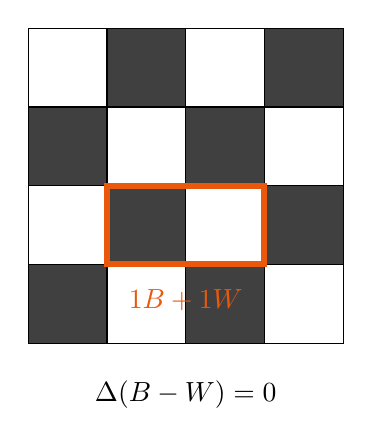
\begin{tikzpicture}
  \foreach \r in {0,...,3}{\foreach \c in {0,...,3}{\pgfmathtruncatemacro{\shade}{mod(\r+\c,2)}\ifnum\shade=0\def\cell{black!75}\else\def\cell{white}\fi\draw[fill=\cell] (\c,\r) rectangle ++(1,1);}}
  \draw[FigureOrange,line width=2.2pt] (1,1) rectangle (3,2);
  \node[FigureOrange] at (2,.55) {$1B+1W$};
  \node at (2,-.65) {$\Delta(B-W)=0$};
\end{tikzpicture}
\end{document}
